\documentclass[11pt,aspectratio=43,usenames,dvipsnames]{beamer}
\usepackage[utf8]{inputenc}
\usepackage{amsmath, amsfonts, amssymb, amsthm}
\usepackage[T1]{fontenc}
% mint: code chuck and syntax highlighting
%% outputdir should change according to pdf build directory
\usepackage[outputdir=build,cache=false]{minted}
\usepackage{lmodern}
\usepackage{xcolor}
\usepackage{setspace}
\usepackage{booktabs}
\usepackage{multirow}
\usepackage{graphicx}
\usepackage{tikz}
% \usetikzlibrary{decorations}
\usetikzlibrary{decorations.pathreplacing, intersections}
\usepackage{ulem}
\usepackage{hyperref}
\usepackage{booktabs}
\usepackage{babel}
\usepackage{makecell}
\usepackage[para,online,flushleft]{threeparttable}
\usepackage{pdfpages}
\usepackage{tcolorbox}
\usepackage{bm}
\usepackage{appendixnumberbeamer}
\usepackage{natbib}
\usepackage{caption}
\captionsetup[figure]{labelformat=empty}% redefines the caption setup of the figures environment in the beamer class.
\usetheme[compress]{Boadilla}
\usecolortheme{default}
\useoutertheme{miniframes}
\usefonttheme[onlymath]{serif}

\newcommand{\jump}[2]{\hyperlink{#1}{\beamerbutton{#2}}}
\newcommand{\orange}[1]{\textcolor{orange}{#1}}
\newcommand{\red}[1]{\textcolor{red}{#1}}
\newcommand{\blue}[1]{\textcolor{blue}{#1}}
\newcommand{\green}[1]{\textcolor{OliveGreen}{#1}}

\renewcommand{\square}{\scalebox{0.7}{$\blacksquare$ \hspace{0.5em}}}
\setbeamertemplate{itemize item}{\raisebox{0.1em}{\scalebox{0.7}{$\blacksquare$}}}
\setbeamertemplate{itemize subitem}[circle]
\setbeamertemplate{itemize subsubitem}{--}
\setbeamercolor{itemize item}{fg=black}
\setbeamercolor{itemize subitem}{fg=black}
\setbeamercolor{itemize subsubitem}{fg=black}
\setbeamercolor{item projected}{bg=darkgray,fg=white}
\definecolor{blue}{rgb}{0.2, 0.2, 0.7}
\setbeamercolor{alerted text}{fg=blue}
\setbeamertemplate{enumerate items}[circle]


\setbeamertemplate{headline}{}

%==========================================
\let\olditemize=\itemize
\let\endolditemize=\enditemize
\renewenvironment{itemize}{\olditemize \itemsep1em}{\endolditemize}
\let\oldenumerate=\enumerate
\let\endoldenumerate=\endenumerate
\renewenvironment{enumerate}{\oldenumerate \itemsep1em}{ \endoldenumerate}

\DeclareMathOperator*{\argmax}{\arg\!\max}
\DeclareMathOperator*{\E}{\mathbb{E}}
\DeclareMathOperator*{\var}{\rm Var}
\DeclareMathOperator*{\cov}{\rm Cov}

\theoremstyle{definition}
\newtheorem{assume}{Assumption}
\newtheorem{lem}{Lemma}
\newtheorem{proposition}{Proposition}
\newtheorem{thm}{Theorem}
\newtheorem{corol}{Corollary}

\AtBeginSection[]{
  \begin{frame}[noframenumbering]
  \vfill
  \centering
  \begin{beamercolorbox}[sep=8pt,center,shadow=true,rounded=true]{title}
    \usebeamerfont{title}\insertsection\par%
  \end{beamercolorbox}
  \vfill
  \end{frame}
}

\begin{document}
    \title[Unit 2]{Unit 2 \\ Technological Change, Population and Growth}
    \author[Hui-Jun Chen]{Hui-Jun Chen}
    \institute[OSU]{The Ohio State University}
    \date{\today}
    \setbeamertemplate{navigation symbols}{}
    \setstretch{1.2}

%-------------------------------------------------------
{
%	\usebackgroundtemplate{\includegraphics[width=1\paperwidth]{../EveningSky_cropped_edit43_bright.jpg}}
    \begin{frame}
% \vspace{3em}
        \centering
%		{\footnotesize 	ECON 4002 Intermediate Macroeconomic Theory}
        \maketitle
% \vspace{-1.5em}
% \centering
% \includegraphics[width=0.55\linewidth]{Pictures/houses.jpeg}


    \end{frame}
}

% -------------------------------------------
\setbeamertemplate{headline}
{
\setbeamercolor{section in head/foot}{fg=black, bg=white}
\vskip1em \tiny \insertsectionnavigationhorizontal{1\paperwidth}{\hspace{0.50\paperwidth}}{}
}
%------------------------------------------

\section[Intro]{Introduction}
\label{sec:Introduction}

\begin{frame}{Economics Reasoning}
\label{slide:Economics_Reasoning}
    \begin{center}
        How could we understand the ``Hocky-stick'' growth?
    \end{center}

    \begin{itemize}
        \item Recall the Interactive figure: \blue{\url{https://tinyco.re/3290463}}
        \item Two facts we want to explain:
        \begin{enumerate}
            \item rapid growth starting from 1800s, and
            \item stagnation in the centries before 1800s
        \end{enumerate}
        \item In econ, we usually use \textbf{model} to understand Economics phenomenon.
        \item We will build two models to explain both facts above.
        \item Further reading: \alert{\url{https://tinyurl.com/4upjz46u}}
    \end{itemize}
\end{frame}

\section[EconModel]{Economics Model}
\label{sec:Economics_Model}

\begin{frame}{Anecdotic Illustration of Economics Model}
\label{slide:Anecdotic_Illustration_of_Economics_Model}

Build your own world (similar to real world) so that you know every detail!

\begin{center}

\includegraphics[width=0.9\textwidth]{./figures/6375692be499513c6f3be825_Minecraft-logo.png}
\end{center}

\end{frame}

\begin{frame}{Formal Illustration of Economics Model}
\label{slide:Formal_Illustration_of_Economics_Model}
    \begin{itemize}
        \item Model is an alternative economy which only the \textit{essential feature} of the economy that are \textbf{relevant to the question} are maintained
        \item To see deeper mechanism in real world, we need \alert{simplification}
        \item Necessary evil to omit many real world details $ \Rightarrow  $ endless debate!
    \end{itemize}

    \begin{center}
    \small
    \begin{tabular}{cc}
        \alert{assumptions}
        \\
        that (we think)
        \\
        matters
    \end{tabular}
    $ \Rightarrow  $
    \begin{tabular}{cc}
        How \alert{agent} act
        \\
        with each other
        \\
        \& assumptions
    \end{tabular}
    $ \Rightarrow  $
    \begin{tabular}{cc}
        Outcome /
        \\
        \alert{Equilibrium}
    \end{tabular}
    $ \Rightarrow  $
    \begin{tabular}{cc}
        Assumptions
        \\
        Changes?
    \end{tabular}
    \end{center}

    \begin{itemize}
        \item \textbf{Equilibrium}: all forces within model are \alert{balanced} unless \textit{external force} is introduced
    \end{itemize}
\end{frame}

\begin{frame}{What makes a good model?}
\label{slide:What_makes_a_good_model_}
    \begin{center}
        \alert{Friedman's critique}: model are judged by \alert{prediction power}
    \end{center}
    \begin{itemize}
        \item Clarity: is the logic and causality understandable?
        \item Prediction power: match data?
        \item Communication: what we (dis-)agree about?
    \end{itemize}

    \vspace{0.7em}

    ALL models are fake, only some are useful, i.e., elucidates the \alert{underlying mechanism} that people implicitly follows

\end{frame}

\begin{frame}{Key concepts}
\label{slide:Key_concepts}
    \begin{itemize}
        \item \alert{Ceteris paribus} and other simplifications help us focus on the variables of interest. We see more by looking at less.
        \item \alert{Incentives} matter, because they affect the benefits and costs of taking one action as opposed to another.
        \item \alert{Relative prices} help us compare alternatives.
        \item \alert{Economic rent} is the basis of how people make choices.
    \end{itemize}
\end{frame}

\section[Growth?]{Why ``Hocky-stick'' Growth?}
\label{sec:Why___Hocky_stick___Growth_}

\begin{frame}{The need to develop technology}
\label{slide:The_need_to_develop_technology}
\begin{itemize}
    \item There are two inputs for textiles: energy (coal) and labor
    \item Britain v.s. France: wage is higher yet coal is cheaper
    \item $ \Rightarrow  $ \alert{incentive} to invent steam machine, lower average cost
    \begin{center}
        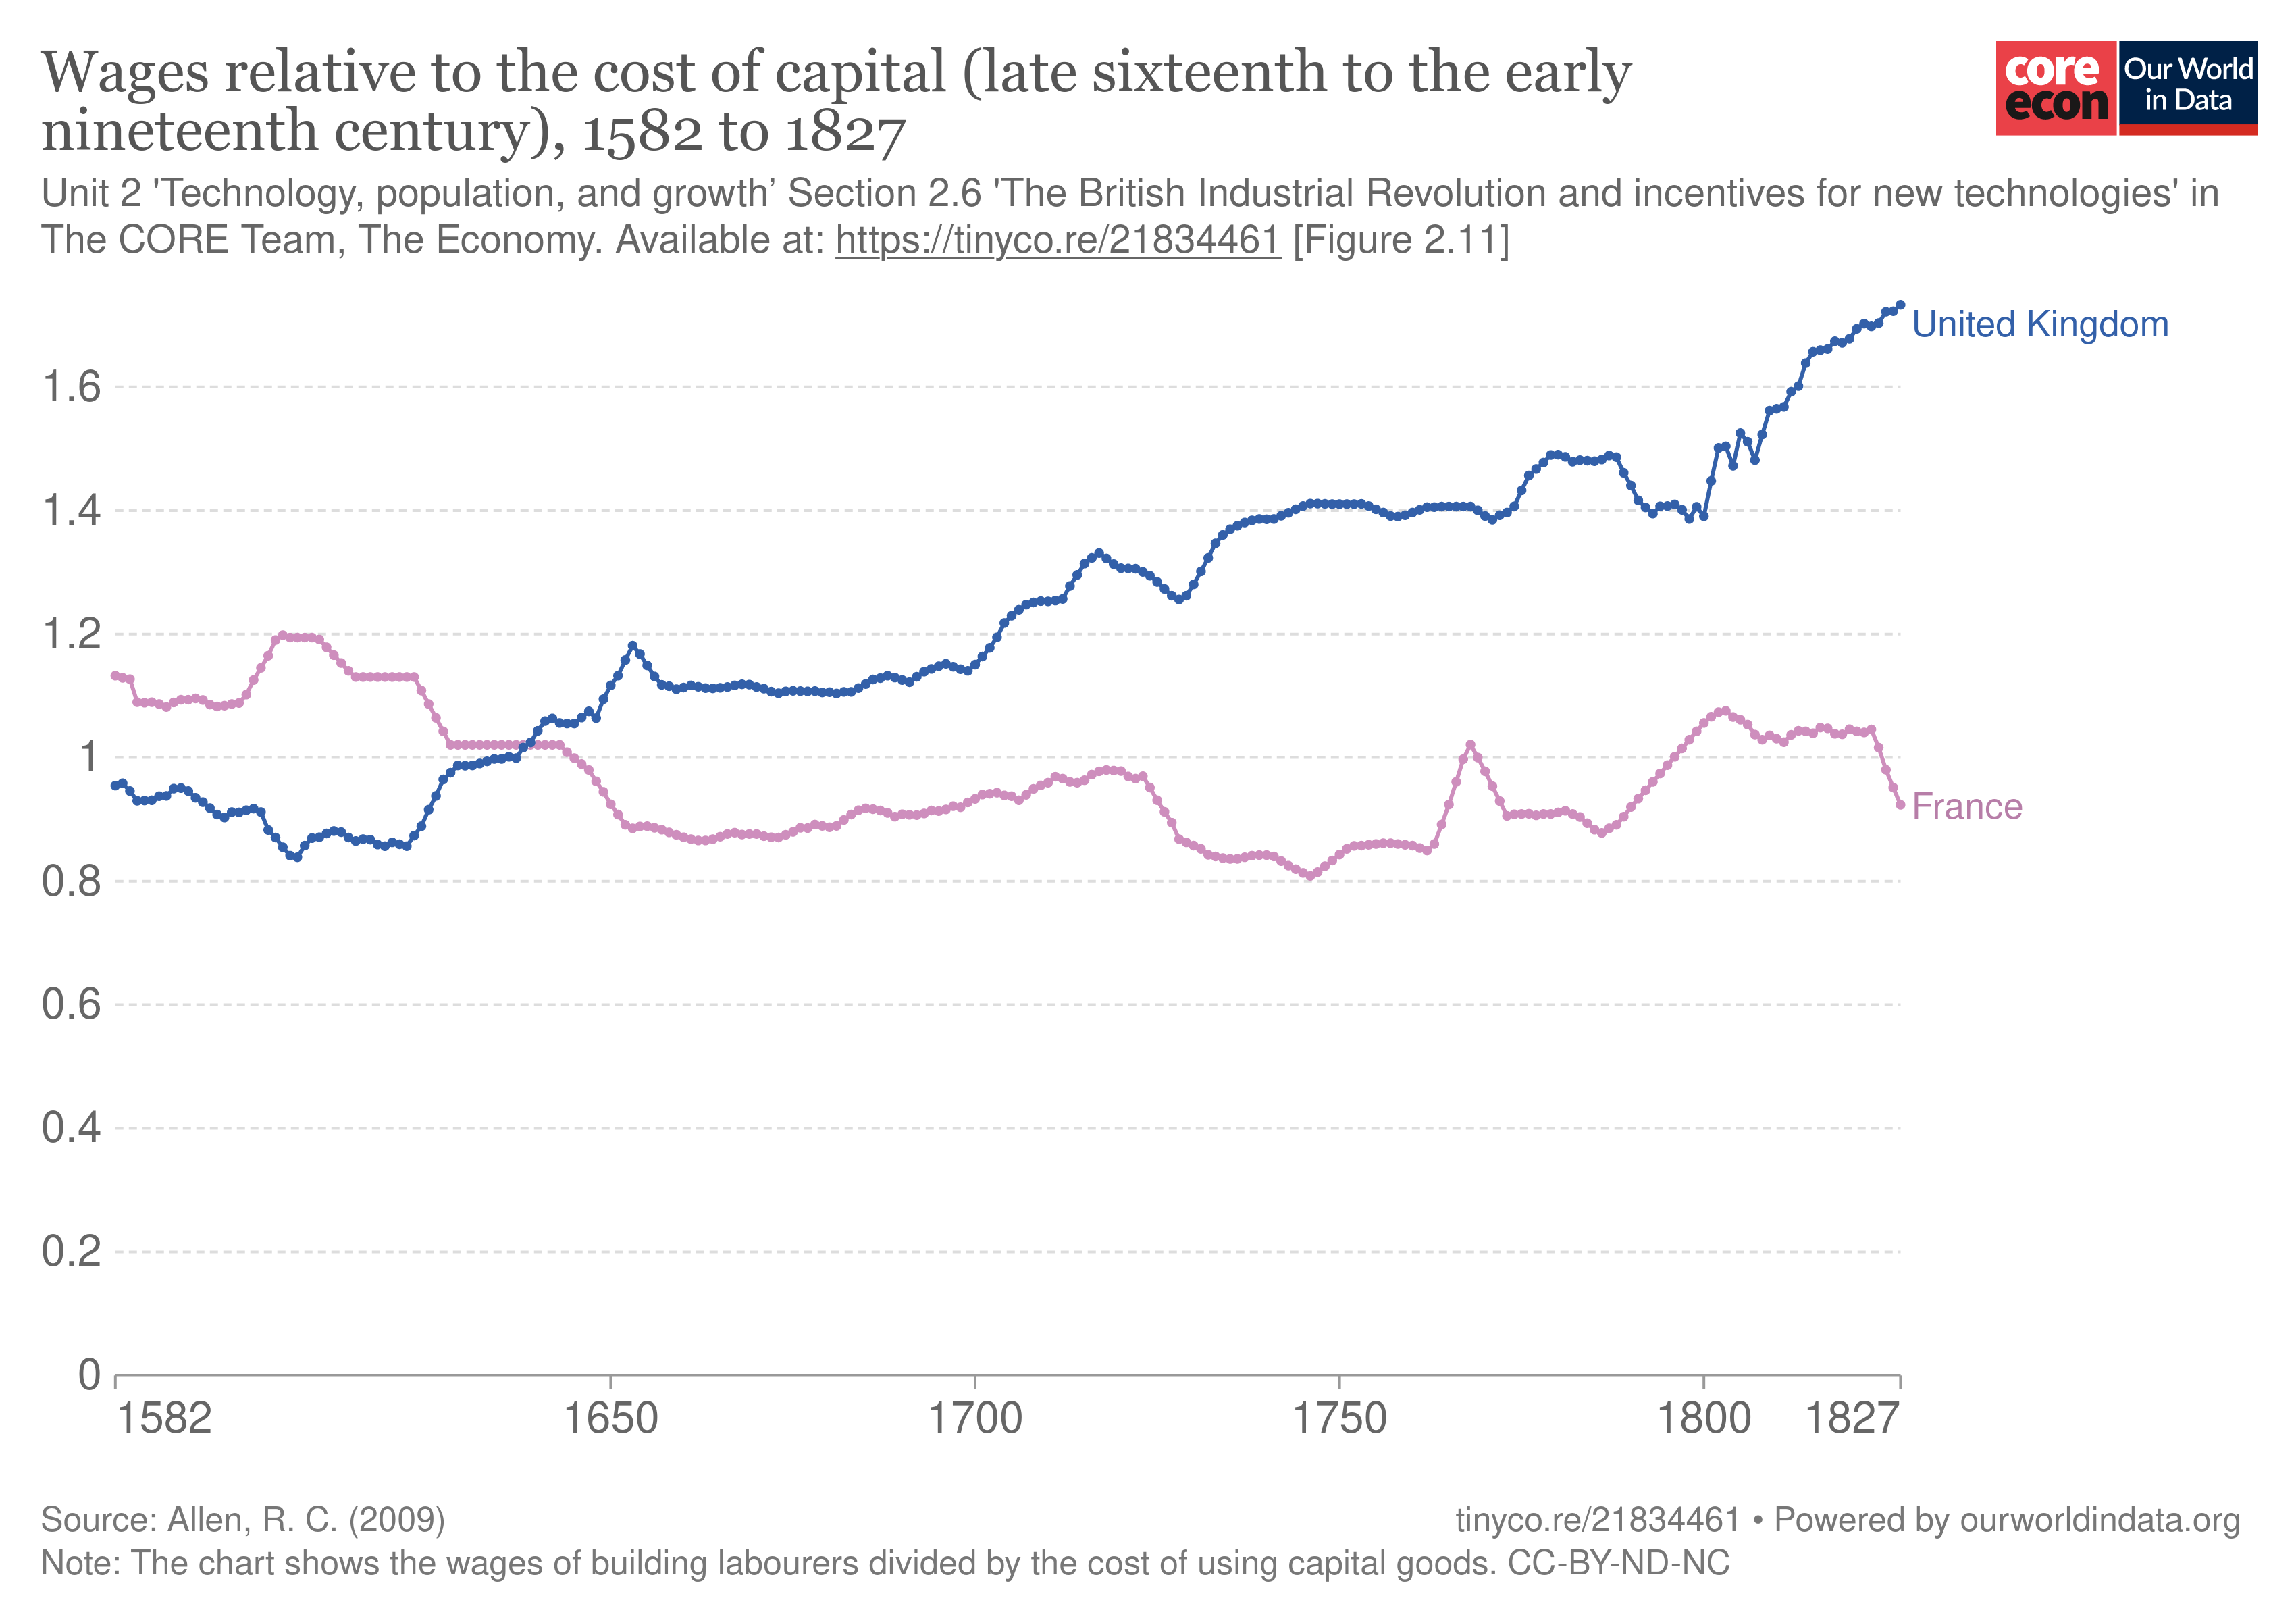
\includegraphics[width=0.6\textwidth]{./figures/wages-relative-to-the-cost-of-capital.png}
    \end{center}
    % \item Steam machine improves the production efficiency, further lower average cost

\end{itemize}
\end{frame}

\begin{frame}{Modelling Technology}
\label{slide:Modelling_Technology}
    \begin{center}
        Inputs $ \underbrace{\Longrightarrow}_{\text{Technology}} $ Outputs
    \end{center}
    \begin{columns}
        \begin{column}{0.4\textwidth}
            \begin{itemize}
                \item All A-E produce 100 cloth
                \item A: relatively energy-intensive
                \item E: relatively labor-intensive
            \end{itemize}
        \end{column}
        \begin{column}{0.6\textwidth}
            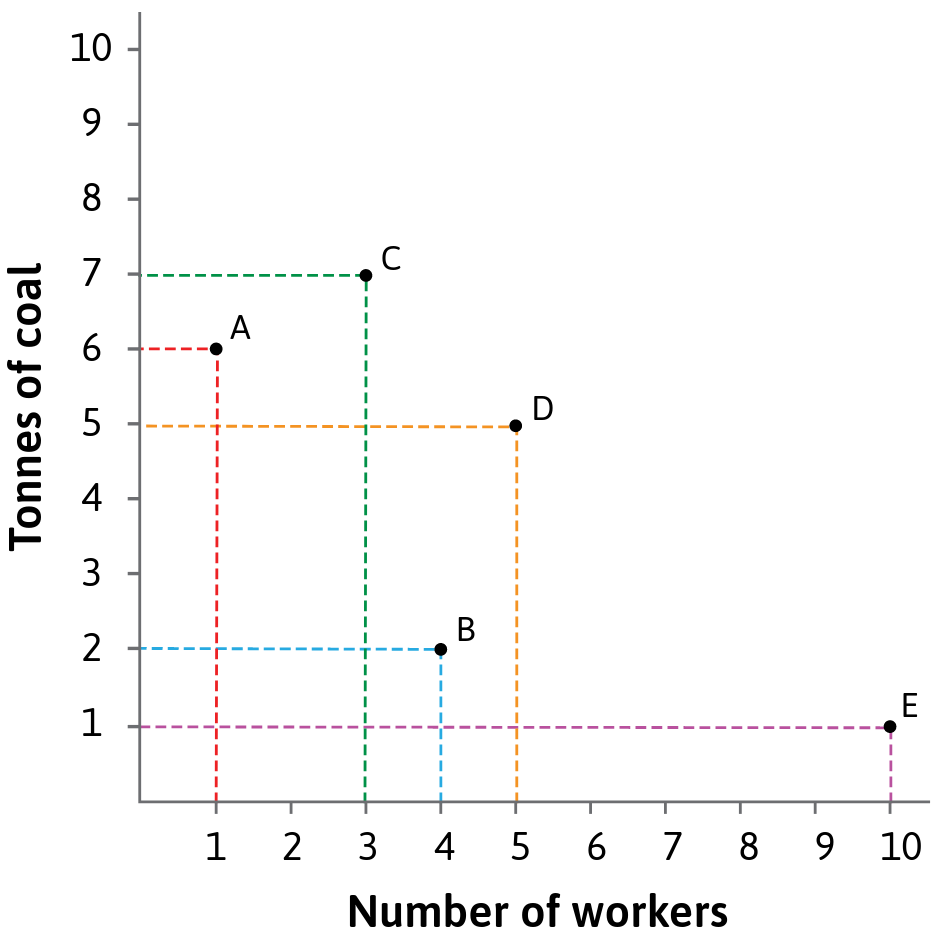
\includegraphics[width=\textwidth]{./figures/Figure2_3.png}
        \end{column}
    \end{columns}

\end{frame}

\begin{frame}{Some Technology are Inferior}
\label{slide:Some_Technology_are_Inferior}
    \begin{columns}
        \begin{column}{0.6\textwidth}
            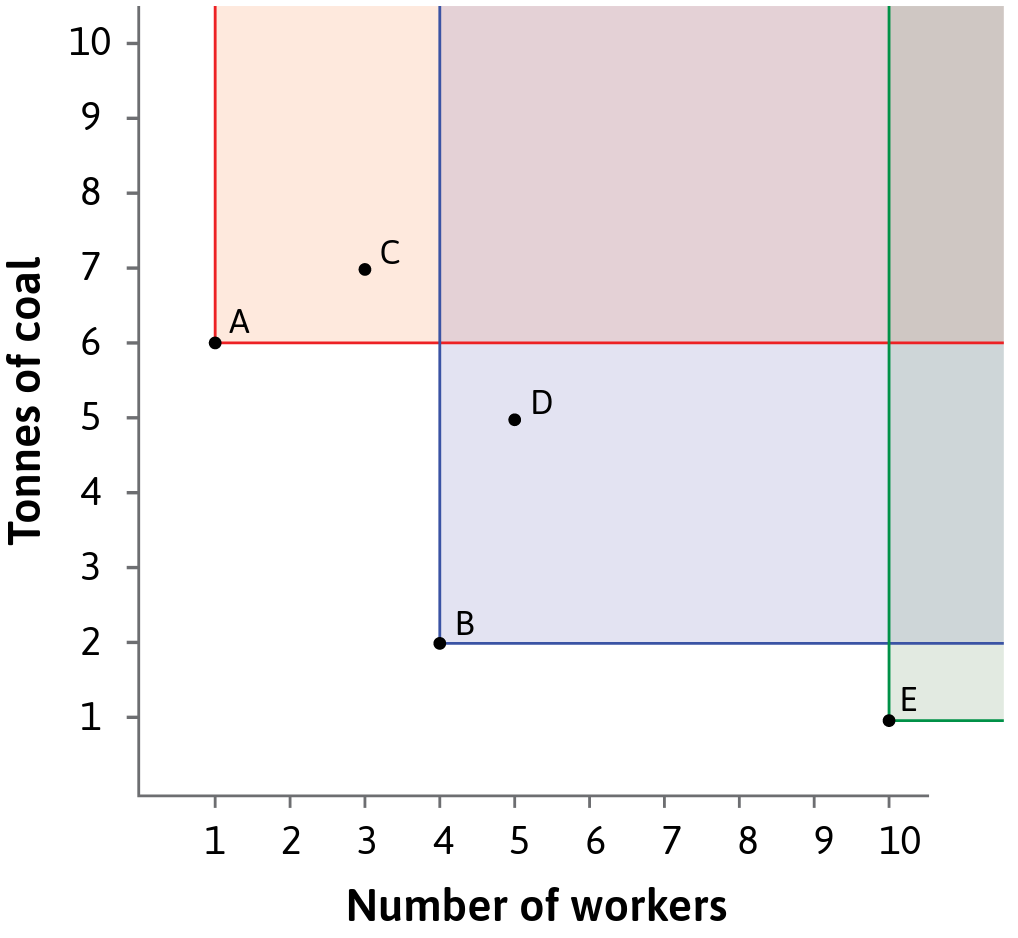
\includegraphics[width=\textwidth]{./figures/Figure2_4.png}
        \end{column}
        \begin{column}{0.4\textwidth}
            \begin{itemize}
                \item Tech C is dominated by A, and Tech D is dominated by B
                \item C produce the same output as A, but use more input
            \end{itemize}
        \end{column}
    \end{columns}

\end{frame}

\begin{frame}{Firm's Behavior}
\label{slide:Firm_s_Behavior}
    \begin{itemize}
        \item Firm's Objective: \alert{maximizing profit} ($\neq$ minimizing cost)
        \item Profit $ = $ revenue $ - $ costs
        \item If revenue if fixed (?!), then \alert{maximizing profit} $=$ minimizing cost
        \item cost $ = $ wage $ \times  $ workers $ + $ price of coal per ton $ \times  $ numbers of ton
        \begin{itemize}
            \item $ c = w \times L + p \times R $
        \end{itemize}
        \item \textbf{Isocost line}: the combination of $ (L, R) $ that yields same cost $ c $, given market prices $ w $ and $ p $
        \item To draw the line, we rearrange the cost function into
        %
        \begin{equation*}
            R = \frac{c}{p} - \underbrace{\frac{w}{p}}_{\text{relative price}} L
        \end{equation*}
        %
    \end{itemize}
\end{frame}

\begin{frame}{Change in relative price}
\label{slide:Change_in_relative_price}
    \begin{columns}
        \begin{column}{0.4\textwidth}
            \begin{itemize}
                \small
                \item Interactive figure: \blue{\url{https://tinyurl.com/2fsfzcm3}}
                \item Original at pt B, with isocost line $\overline{JH}$,  $ \displaystyle  \frac{w}{p} = \frac{10}{20} = \frac{1}{2} $
                \item Relative price increases such that $ \displaystyle \frac{w}{p} = \frac{10}{5} = 2 $, isocost line steeper
                \item Cost increase if still stay at labor-intensive tech B $ \Rightarrow  $ move to energy-intensive tech A
            \end{itemize}
        \end{column}
        \begin{column}{0.6\textwidth}
            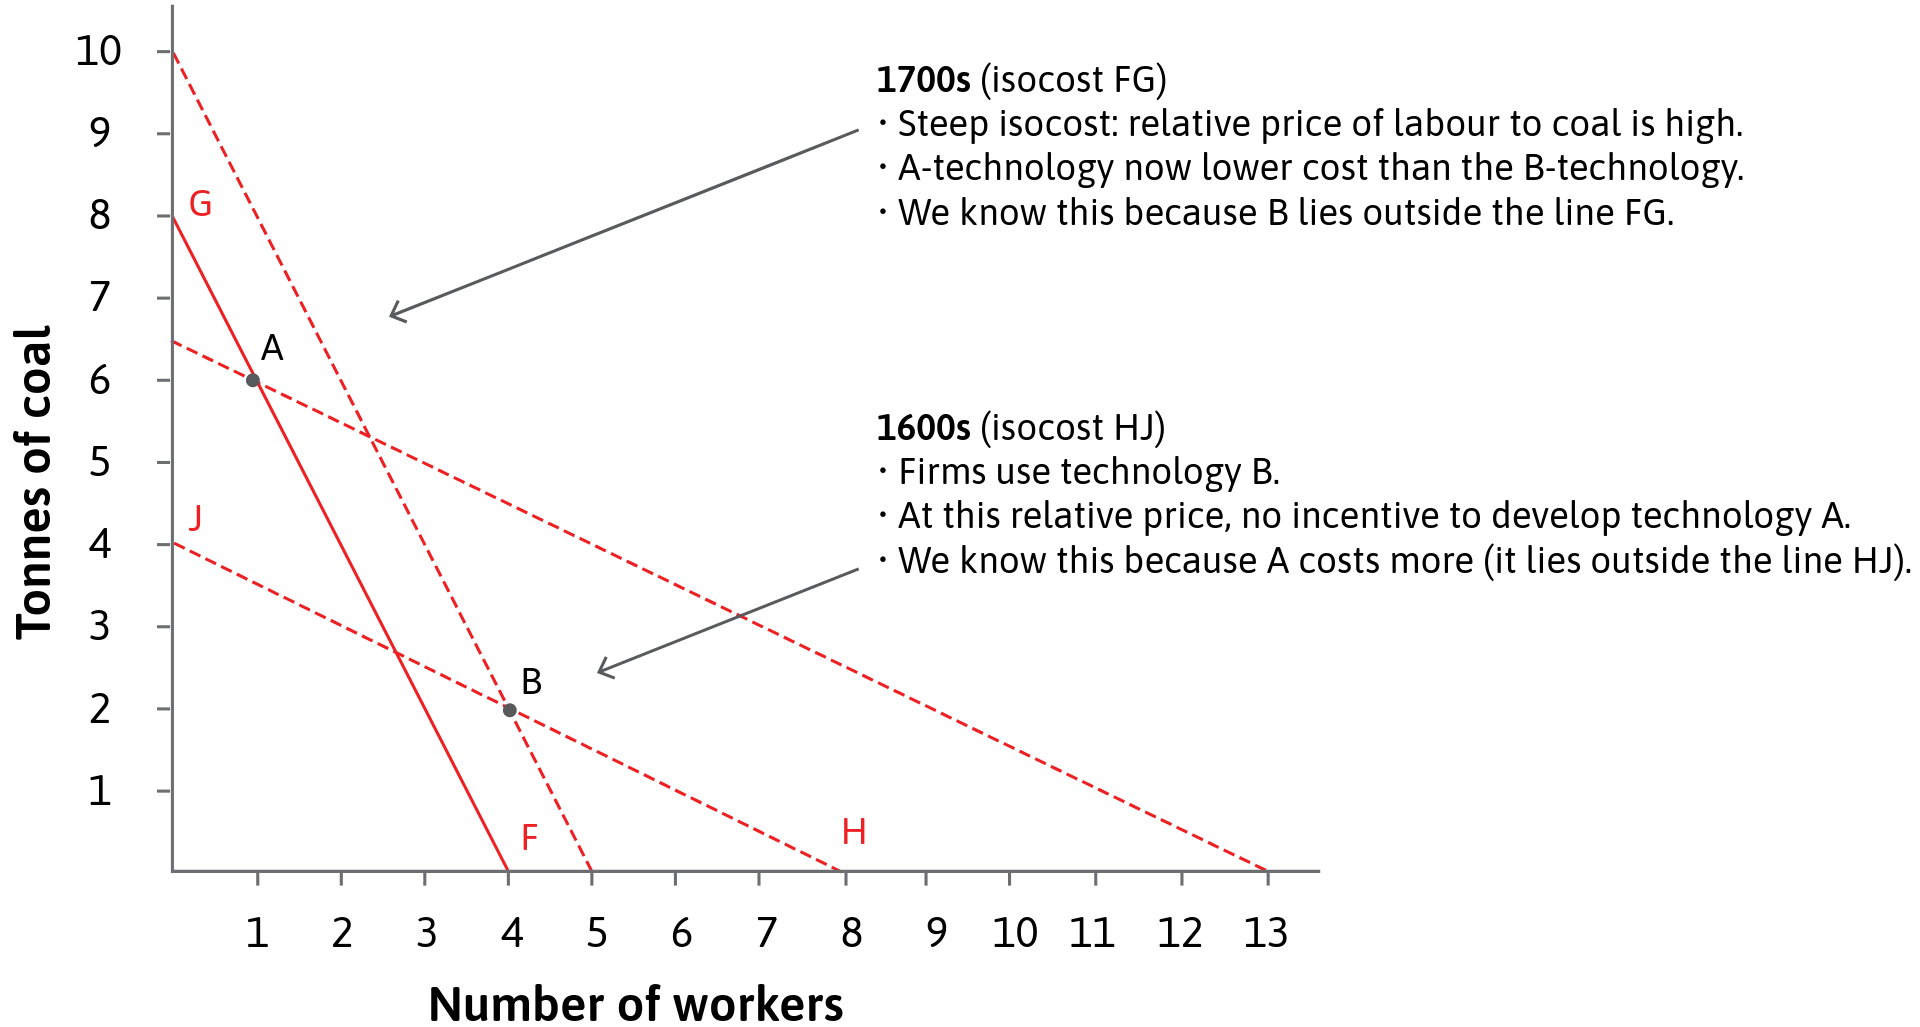
\includegraphics[width=\textwidth]{./figures/Figure2_12.png}
        \end{column}
    \end{columns}
\end{frame}

\section[Stagnation?]{Why Stagnation?}
\label{sec:Why_Stagnation_}

\begin{frame}{Malthusian Trap}
\label{slide:Malthusian_Trap}
    \begin{itemize}
        \item Law of diminishing return: increment of output $ \downarrow  $ as input $ \uparrow $
        \begin{itemize}
            \item e.g. Study effort is lower from 50 $ \rightarrow  $ 60 compared with 90 $ \rightarrow  $ 100
        \end{itemize}
        \item Production function also exhibit \alert{diminishing average product of labor}:
    \end{itemize}

    \begin{center}
    \begin{tabular}{ c c c }
        Harvest more
            & $ \Rightarrow $
            & Farmer income $ \uparrow  $
        \\
        $ \Uparrow \text{(random)}  $
            &
            & $ \Downarrow $
        \\
        Population $ \downarrow  $
            &
            & Living standard \& Population $ \uparrow  $
        \\
        $ \Uparrow  $
            &
            & $ \Downarrow $
        \\
        Farmer income $ \downarrow  $
            & $ \Leftarrow  $
            & Limited land cause average return $ \downarrow  $
        \\
    \end{tabular}
    \end{center}

\end{frame}

\begin{frame}{O Fortuna! (Carmina Burana)}
\label{slide:O_Fortuna_}
    \begin{center}
        \includegraphics[width=0.8\textwidth]{./figures/CarminaBurana_wheel.jpg}
    \end{center}
\end{frame}

\begin{frame}{Was Malthus Correct?}
\label{slide:Was_Malthus_Correct_}
    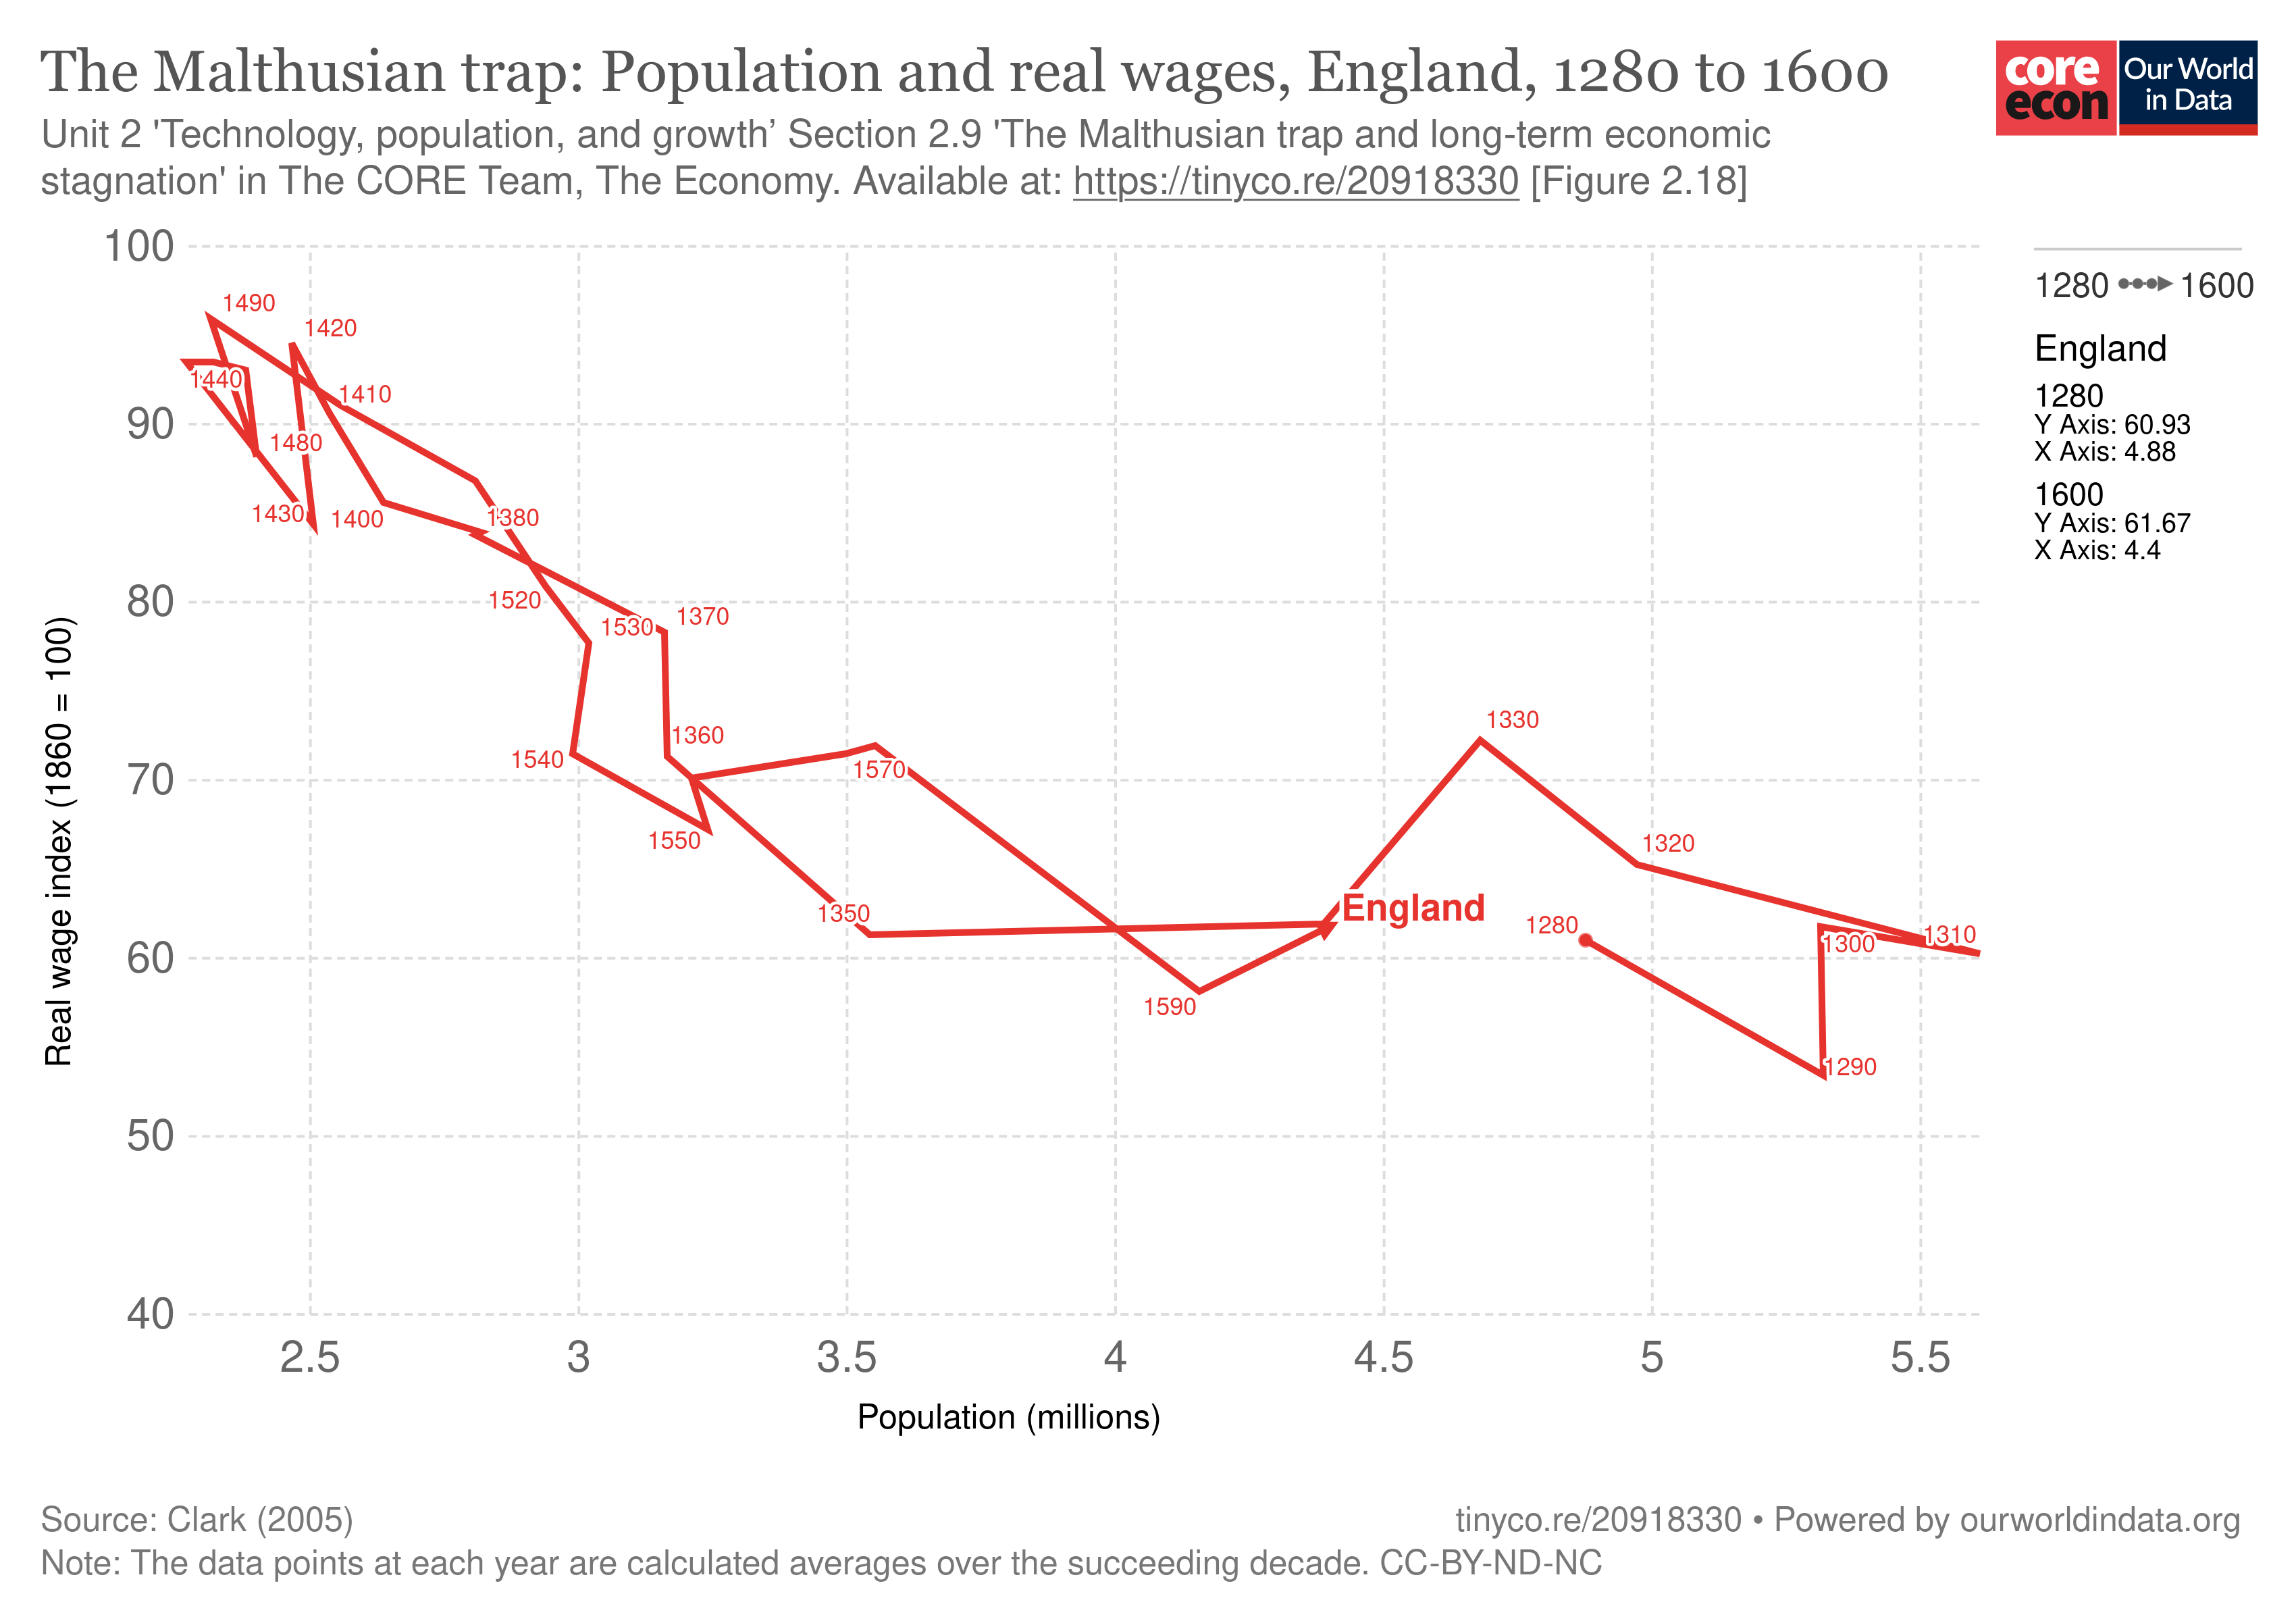
\includegraphics[width=0.95\textwidth]{./figures/the-malthusian-trap.png}
\end{frame}

\begin{frame}{How could we escape from Malthusian trap?}
\label{slide:How_could_we_escape_from_Malthusian_trap_}
    By \alert{improvement in technology} to offset diminishing return!

    \begin{center}
        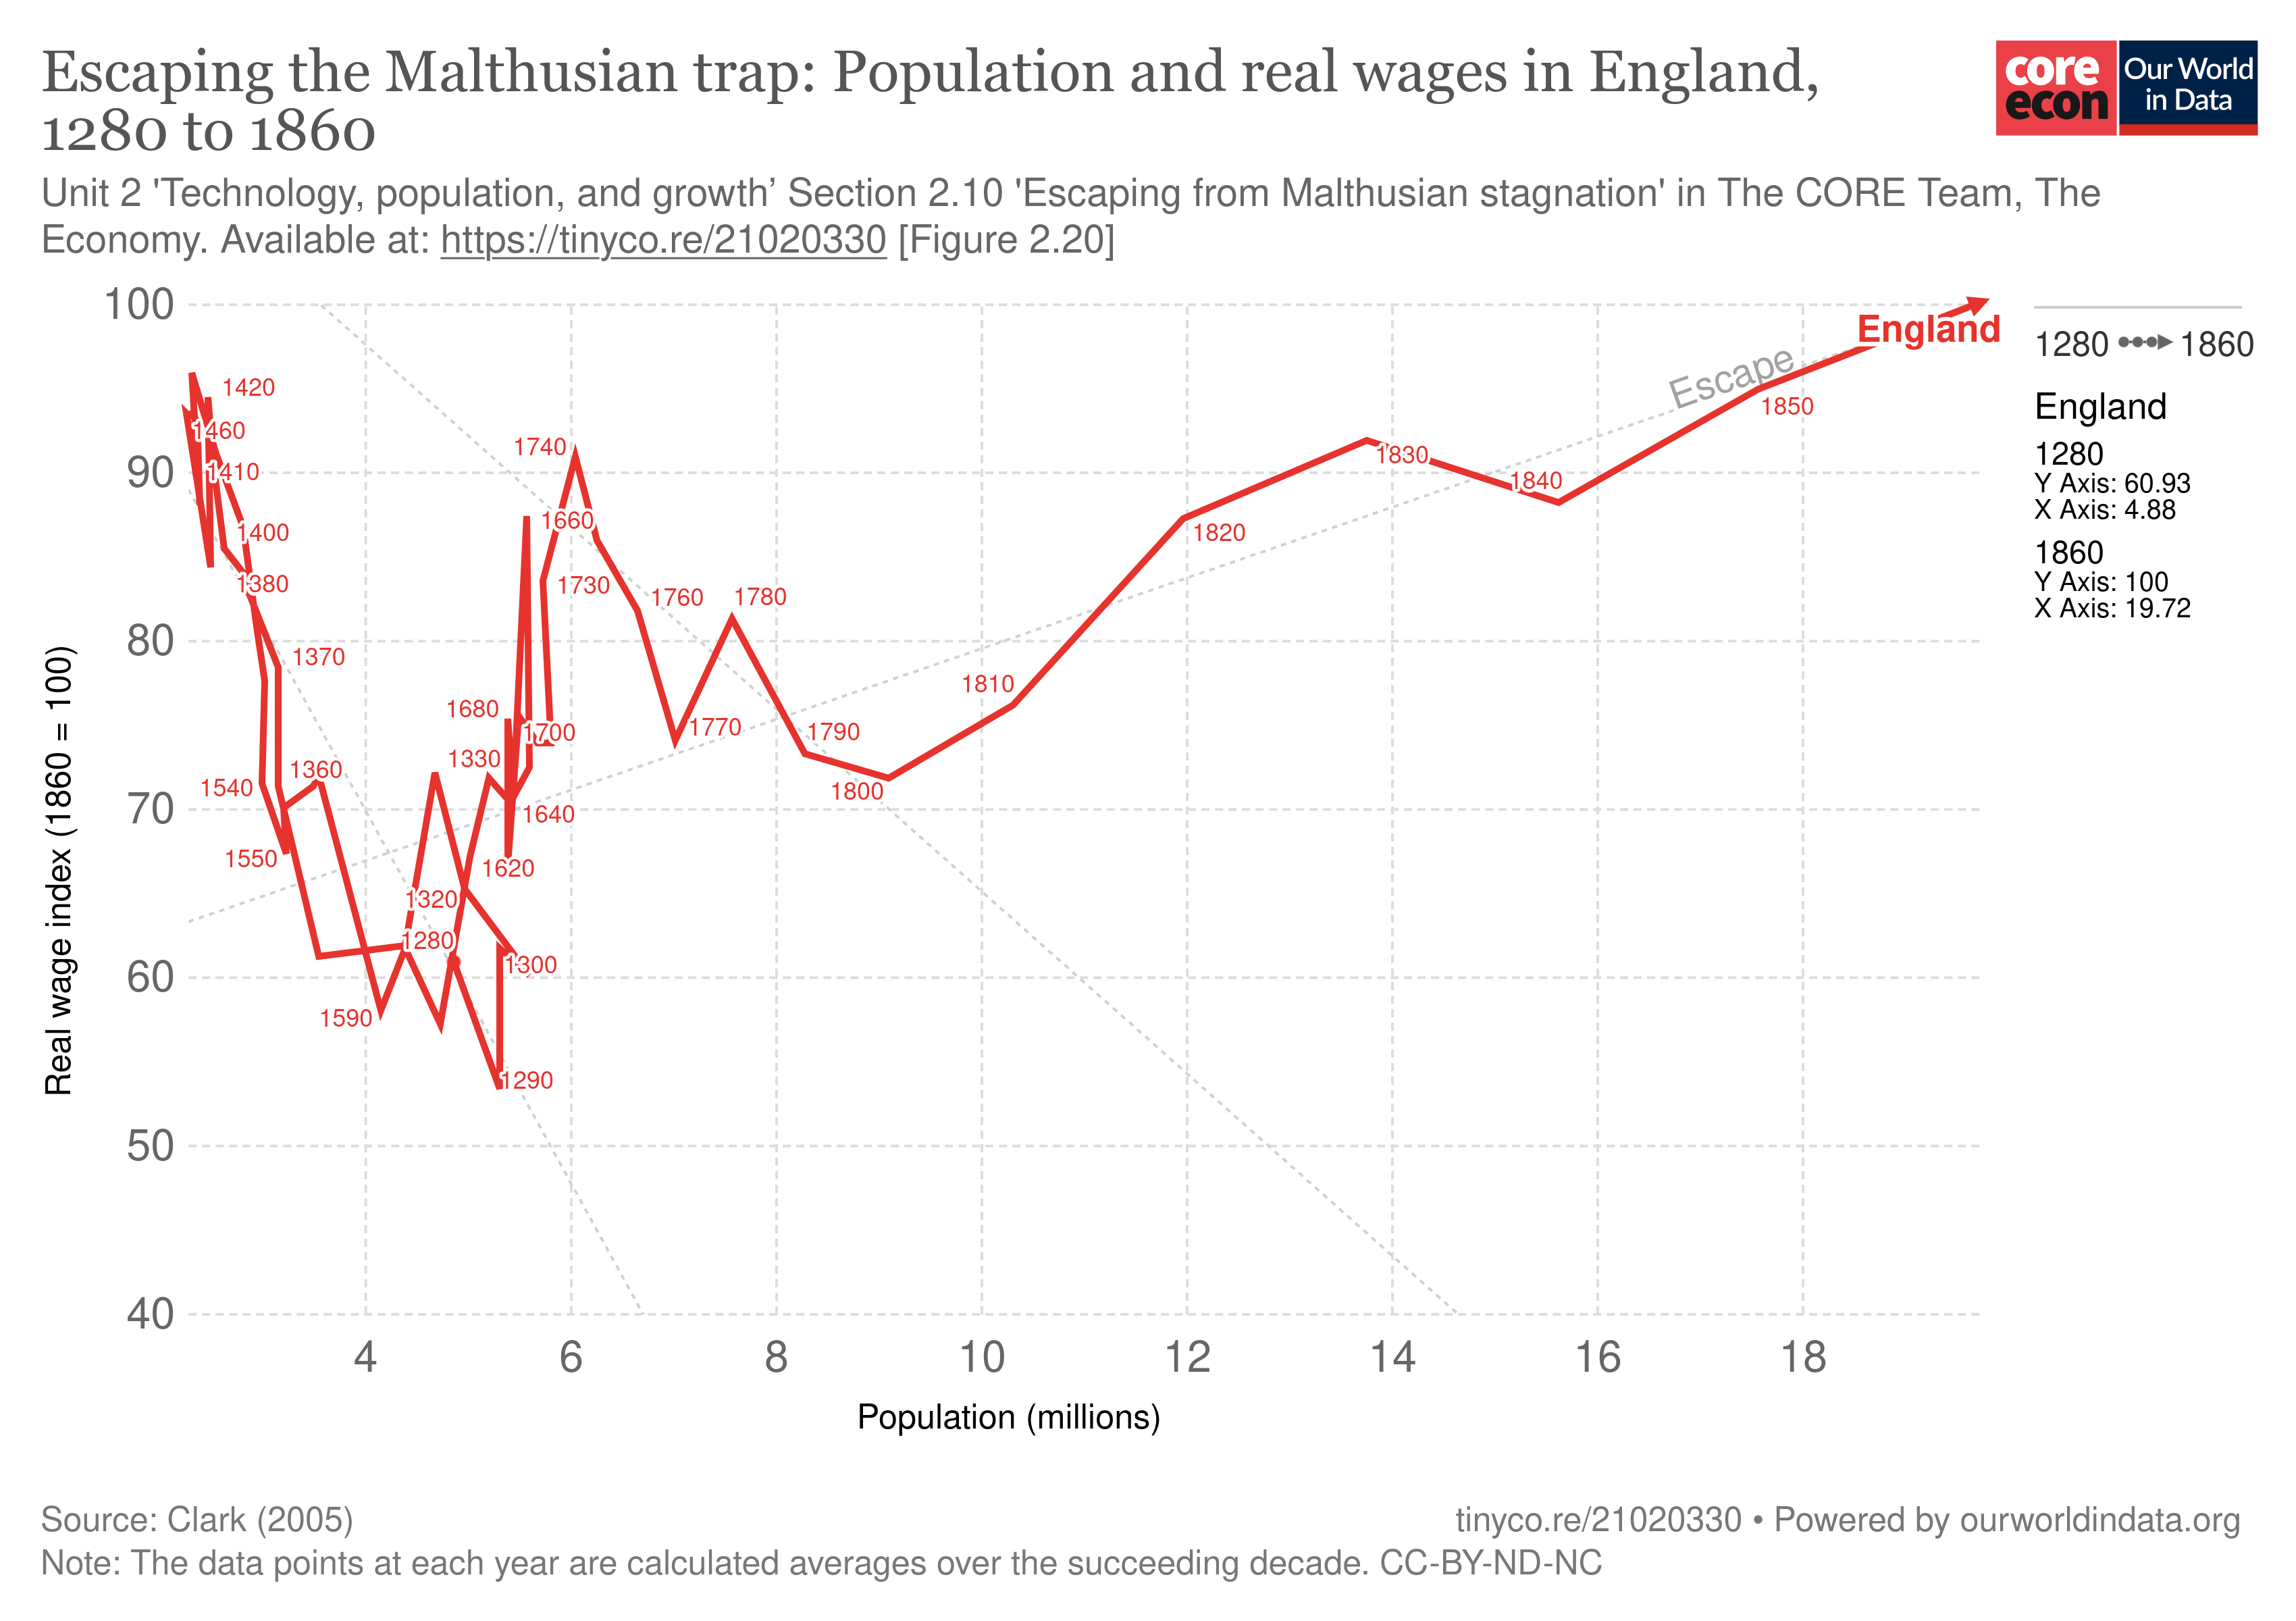
\includegraphics[width=0.9\textwidth]{./figures/escaping-the-malthusian-trap.png}
    \end{center}
\end{frame}

\end{document}
